% =====================================================================
%  Redes Neuronales 2026 (FaMAF-UNC) - Trabajo Práctico 1
%  "Simulación numérica del modelo de neuronas de Izhikevich"
%  Consigna vigente: tp1-2026-actualizado.pdf (28/9/2026). Límite: 4 páginas.
%
%  De dónde sale cada número:
%   - Primera parte: notebook del grupo (TP1-Izhikevich.ipynb) y
%     tp1-izhikevich/tp1_izhikevich.ipynb, que dan los mismos tiempos de disparo.
%   - Error numérico y red: tp1-izhikevich/codigo/resultados.json (semilla 2026).
%  Figuras en figuras/. Compilar con pdfLaTeX (en Overleaf: Recompile).
%  Falta completar: los nombres de los autores (entre [corchetes]).
% =====================================================================
\documentclass[10pt,a4paper,twocolumn]{article}

\usepackage[utf8]{inputenc}
\usepackage[T1]{fontenc}
\usepackage[spanish,es-tabla,es-noshorthands]{babel}
\usepackage{lmodern}
\usepackage[a4paper,margin=1.7cm,columnsep=0.65cm]{geometry}
\usepackage{microtype}
\usepackage{amsmath,amssymb}
\usepackage{siunitx}
\sisetup{output-decimal-marker={,},group-minimum-digits=5}
\DeclareSIUnit{\milivolt}{mV}
\usepackage{graphicx}
\graphicspath{{figuras/}}
\usepackage{booktabs}
\usepackage[font=small,labelfont=bf,skip=4pt]{caption}
\usepackage{xcolor}
\usepackage[colorlinks=true,linkcolor=blue!50!black,citecolor=blue!50!black,urlcolor=blue!50!black]{hyperref}

\setlength{\textfloatsep}{8pt plus 2pt minus 2pt}
\setlength{\floatsep}{6pt plus 2pt minus 2pt}
\setlength{\dbltextfloatsep}{8pt plus 2pt minus 2pt}

% =====================================================================
\title{\vspace{-1.2cm}\textbf{Simulación numérica del modelo de neuronas de Izhikevich}}
\author{%
  [Nombre Apellido 1], [Nombre Apellido 2], [Nombre Apellido 3]\\[2pt]
  \small Facultad de Matemática, Astronomía, Física y Computación, Universidad Nacional de Córdoba\\
  \small Redes Neuronales 2026 -- Trabajo Práctico 1
}
\date{\vspace{-0.6cm}}

\raggedbottom
\begin{document}

\twocolumn[{
  \begin{@twocolumnfalse}
    \maketitle
    \vspace{-0.4cm}
    \begin{abstract}
    \noindent
    Estudiamos numéricamente el modelo de neuronas de Izhikevich, un sistema de dos
    ecuaciones diferenciales con una regla de reseteo que reproduce la variedad de
    patrones de disparo de neuronas corticales y talámicas con un costo computacional
    bajo. Integramos el modelo con Runge--Kutta de orden~4 (paso $h=\num{0.1}$\,ms),
    verificando después de cada paso si $v\geq\SI{30}{\milivolt}$ para registrar el
    spike y aplicar el reseteo. Reproducimos cualitativamente los ocho paneles de la
    figura~2 del artículo original (RS, IB, CH, FS, TC con dos protocolos, RZ y LTS) y
    mostramos que, por el tratamiento discreto del reseteo, el error en los tiempos de
    disparo de RK4 decrece sólo linealmente con $h$. En la segunda parte traducimos a
    Python el programa de la red de 1000 neuronas del artículo: obtenemos actividad
    asincrónica de $\approx\num{7.8}$\,Hz con episodios de sincronización, y
    verificamos que eliminar las autoconexiones no cambia la dinámica colectiva.
    Finalmente comparamos dos variantes opcionales: ruido blanco continuo integrado
    con Euler--Maruyama y un acoplamiento continuo mediante $z(v)$.
    \end{abstract}
    \vspace{0.4em}
  \end{@twocolumnfalse}
}]

% =====================================================================
\section{Introducción}
La modelización matemática y computacional es una herramienta fundamental para
estudiar el sistema nervioso: al integrar conocimientos de las neurociencias, la
matemática y la física, permite describir la actividad neuronal y explorar los
mecanismos que la sustentan. Un modelo más detallado no es necesariamente
superior: los modelos deben actuar como puentes entre niveles de comprensión,
con detalle suficiente para vincularse con los mecanismos biológicos y la
simplicidad necesaria para obtener resultados claros~\cite{dayan2001}.

Este equilibrio se observa en los modelos de neurona de disparo, que describen la
evolución del potencial de membrana y la generación de potenciales de acción
(\emph{spikes}) en respuesta a corrientes de entrada. Los modelos
\emph{integrate-and-fire}, derivados de la propuesta de Lapicque~\cite{lapicque1907},
integran las corrientes de entrada y representan el disparo mediante un umbral y un
posterior reseteo del potencial: al omitir la forma del potencial de acción facilitan
el análisis matemático y reducen el costo computacional~\cite{dayan2001}, pero no
producen la riqueza de patrones de disparo de las neuronas
corticales~\cite{izhikevich2003}. El modelo de Hodgkin y Huxley~\cite{hodgkin1952},
en cambio, describe explícitamente las conductancias de sodio y potasio dependientes
del voltaje, a costa de un sistema de ecuaciones más complejo, cuyo costo lo vuelve
prohibitivo para simular redes grandes~\cite{izhikevich2003}.

El modelo de Izhikevich~\cite{izhikevich2003,izhikevich2007} combina ambas
propiedades: es tan eficiente como un \emph{integrate-and-fire} y, variando sólo
cuatro parámetros, reproduce los tipos de disparo conocidos de neuronas corticales y
talámicas. Se obtiene reduciendo modelos de tipo Hodgkin--Huxley mediante teoría de
bifurcaciones y formas normales~\cite{izhikevich2003,izhikevich2007}, y permite
simular en tiempo real redes de miles de neuronas~\cite{izhikevich2003}.

El objetivo de este informe es integrar numéricamente el modelo, reproducir los tipos
de disparo de la figura~2 de la Ref.~\cite{izhikevich2003}, analizar la precisión del
método numérico y estudiar la dinámica colectiva de la red de 1000 neuronas propuesta
en el mismo artículo.

% =====================================================================
\section{Teoría}
\subsection{El modelo de Izhikevich}
Con la notación del artículo original~\cite{izhikevich2003}, $v$ en mV y $t$ en ms,
\begin{align}
  \dot v &= \num{0.04}\,v^2 + 5\,v + 140 - u + I(t), \label{eq:v}\\
  \dot u &= a\,(b\,v - u), \label{eq:u}
\end{align}
con la condición de reseteo
\begin{equation}
  \text{si } v \geq \SI{30}{\milivolt}: \qquad v \leftarrow c, \qquad u \leftarrow u + d .
  \label{eq:reset}
\end{equation}
La variable $v$ es el potencial de membrana y $u$ una variable de recuperación que
resume de manera efectiva procesos iónicos lentos (activación de corrientes de K$^+$ e
inactivación de corrientes de Na$^+$) y aporta realimentación negativa sobre
$v$~\cite{izhikevich2003}. La entrada $I(t)$ representa una corriente inyectada o una
entrada sináptica efectiva. El parámetro $a$ es la escala temporal de recuperación de
$u$ (valores chicos, recuperación lenta); $b$ mide cuánto responde $u$ a las
variaciones subumbrales de $v$; $c$ es el valor de reseteo de $v$ después de un spike,
y $d$ el incremento de $u$ tras cada spike.

El valor $v=\SI{30}{\milivolt}$ es el que usa el algoritmo para registrar el pico del
spike y aplicar el reseteo; \emph{no} es un umbral fisiológico fijo. En este modelo la
iniciación del spike depende del estado previo de $v$ y $u$: según la historia del
potencial, el umbral efectivo va de $\approx-55$ a
$\approx\SI{-40}{\milivolt}$~\cite{izhikevich2003}. Para $I$ constante, el reposo es la
raíz menor de $\num{0.04}v^2+(5-b)v+140+I=0$, con $u^*=b\,v^*$; para $b=\num{0.2}$ e
$I=0$ resulta $v^*=\SI{-70}{\milivolt}$. Si $b<a$ el reposo se pierde por una
bifurcación silla-nodo y si $b>a$, por una de Andronov--Hopf~\cite{izhikevich2003}:
para $a=\num{0.02}$, $b=\num{0.2}$ el reposo deja de ser estable en $I\approx\num{3.8}$
(Hopf), antes de la silla-nodo en $I=4$.

\subsection{Método numérico}
Con $\mathbf{x}=(v,u)$ y $\dot{\mathbf{x}}=\mathbf{f}(t,\mathbf{x})$ usamos Runge--Kutta
de orden~4,
$\mathbf{x}_{n+1} = \mathbf{x}_n + \tfrac{h}{6}(\mathbf{k}_1 + 2\mathbf{k}_2 + 2\mathbf{k}_3 + \mathbf{k}_4)$,
con $\mathbf{k}_1=\mathbf{f}(t_n,\mathbf{x}_n)$,
$\mathbf{k}_{2}=\mathbf{f}(t_n+\tfrac h2,\mathbf{x}_n+\tfrac h2\mathbf{k}_{1})$,
$\mathbf{k}_{3}=\mathbf{f}(t_n+\tfrac h2,\mathbf{x}_n+\tfrac h2\mathbf{k}_{2})$ y
$\mathbf{k}_4=\mathbf{f}(t_n+h,\mathbf{x}_n+h\mathbf{k}_3)$, con $h=\num{0.1}$\,ms.
Después de cada paso se verifica si $v_{n+1}\geq\SI{30}{\milivolt}$; si se cumple, se
registra un spike en $t_{n+1}$ y se aplica inmediatamente el reseteo~\eqref{eq:reset}.
Siempre $u(0)=b\,v(0)$. Como el valor guardado en ese paso ya es $c$, en las figuras se
inserta el pico en \SI{30}{\milivolt}.

\subsection{Red de neuronas}
La red de la sección~IV de la Ref.~\cite{izhikevich2003} tiene $N_e=800$ neuronas
excitatorias y $N_i=200$ inhibitorias regidas por~\eqref{eq:v}--\eqref{eq:reset}, con
parámetros heterogéneos ($r_i\sim U(0,1)$): $a_i=\num{0.02}$, $b_i=\num{0.2}$,
$c_i=-65+15r_i^2$, $d_i=8-6r_i^2$ en las excitatorias (de RS a CH) y
$a_i=\num{0.02}+\num{0.08}r_i$, $b_i=\num{0.25}-\num{0.05}r_i$, $c_i=-65$, $d_i=2$ en las
inhibitorias (de LTS a FS). Los pesos son $S=[\,\num{0.5}R_E\mid -R_I\,]$, con $R_E$ y
$R_I$ uniformes en $[0,1]$ y $s_{ij}$ el peso de la neurona $j$ a la $i$. En cada paso
de 1\,ms la entrada es $I_i=I_i^{\rm ext}+I_i^{\rm syn}$, con ruido talámico
$I_i^{\rm ext}=5\xi_i$ (excitatorias) o $2\xi_i$ (inhibitorias), $\xi_i\sim N(0,1)$, y
acoplamiento por pulsos $I_i^{\rm syn}=\sum_{j\in F}s_{ij}$, donde $F$ son las neuronas
que dispararon; $v$ se actualiza con dos pasos de Euler de \num{0.5}\,ms y $u$ con uno
de 1\,ms. La matriz $S$ es densa y su diagonal no se anula: hay autoconexiones
$s_{ii}\neq0$.

\emph{Variante de Euler--Maruyama.} Entre spikes,
$dV_i=(\num{0.04}V_i^2+5V_i+140-U_i)\,dt+\sigma_i\,dW_i$ y $dU_i=a_i(b_iV_i-U_i)\,dt$, con
$\sigma_i=5$ o 2, manteniendo por separado los saltos sinápticos y el reseteo. El
esquema es $Y_{n+1}=Y_n+f(Y_n)\,h+\sigma\sqrt h\,\xi_n$~\cite{em}: el incremento de
Wiener en un paso $h$ tiene varianza $h$, de ahí el factor $\sqrt h$. En la
reproducción literal del Matlab ese factor \emph{no} corresponde, porque allí el ruido
es una corriente discreta que se sortea una vez por milisegundo, no un proceso de
Wiener.

\emph{Variante con $z(v)$.} Proponemos reemplazar el acoplamiento por pulsos por la
corriente continua $I_i^{\rm syn}(t)=\sum_j s_{ij}\,z(v_j(t))$, con
$z(v)=(87+v)/450-\num{0.0193}$ y $v$ recortado en 30\,mV, dejando todo lo demás igual.
$z(v)$ no es un detector de spikes: en el reposo vale $\approx\num{0.03}$, así que cada
neurona recibe una entrada de fondo permanente. Es un modelo distinto del de la
figura~3 y lo usamos sólo como experimento comparativo.

% =====================================================================
\section{Resultados}

\begin{figure}[t]
  \centering
  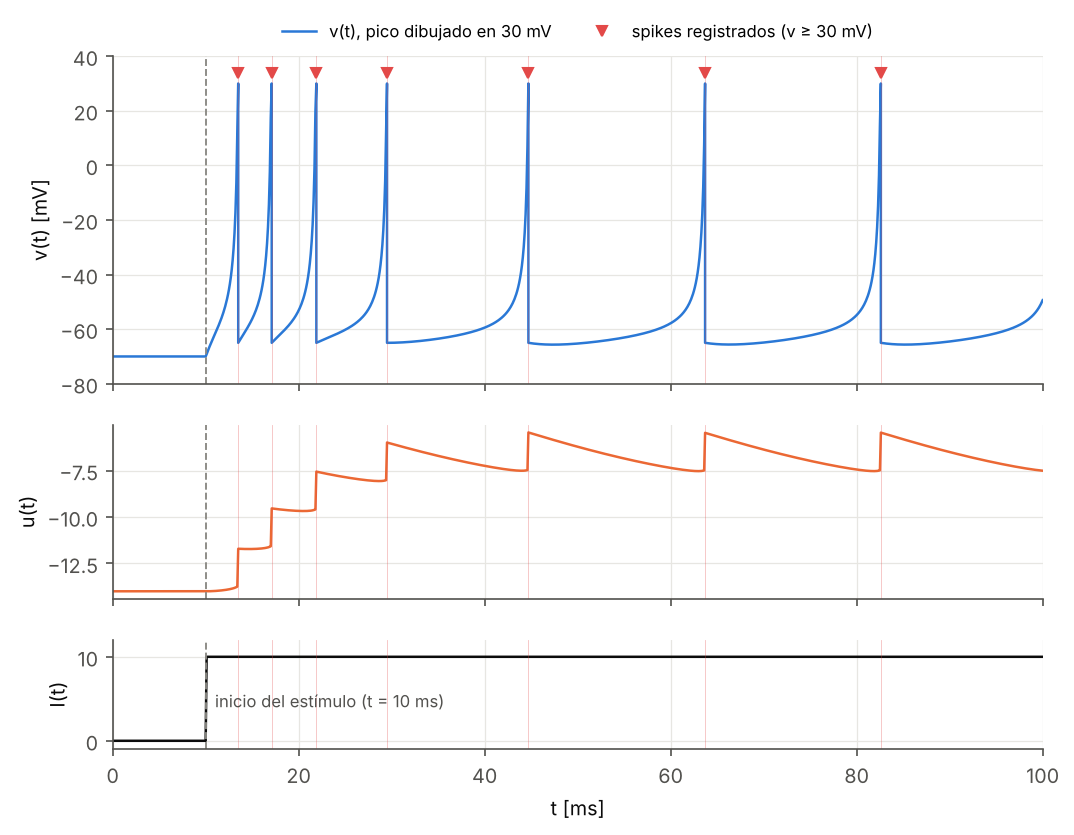
\includegraphics[width=\columnwidth]{f1_base.png}
  \caption{Evolución temporal del potencial de membrana $v(t)$ (arriba, azul), de la
  variable de recuperación $u(t)$ (medio, naranja) y de la corriente $I(t)$ (abajo)
  para $a=\num{0.02}$, $b=\num{0.2}$, $c=\SI{-65}{\milivolt}$, $d=2$, con
  $v(0)=\SI{-70}{\milivolt}$, $u(0)=-14$, RK4 y $h=\num{0.1}$\,ms. La línea discontinua
  marca el inicio del estímulo ($t=10$\,ms); los triángulos y las líneas rojas, los
  tiempos de disparo registrados.}
  \label{fig:base}
\end{figure}

\textbf{Caso base.} En la Figura~\ref{fig:base}, mientras $I=0$ la neurona permanece
en reposo en $v=\SI{-70}{\milivolt}$, $u=-14$. Tras el escalón $I=10$ en $t=10$\,ms
emite siete spikes, en $t=\num{13.5}$, \num{17.1}, \num{21.9}, \num{29.5}, \num{44.7},
\num{63.7} y \num{82.6}\,ms. Los intervalos entre spikes (ISI) crecen de \num{3.6} a
\num{15.2}\,ms y luego se estabilizan en $\approx19$\,ms ($\approx53$\,Hz). La
variable $u$ salta $d=2$ en cada spike y decae entre spikes: su nivel sube durante los
primeros disparos y después oscila entre valores fijos.

\begin{table}[t]
  \centering
  \caption{Parámetros (notación de la Ref.~\cite{izhikevich2003}), corriente de entrada,
  potencial inicial (con $u(0)=b\,v(0)$) y número de spikes obtenidos en cada panel.}
  \label{tab:parametros}
  \small\setlength{\tabcolsep}{4pt}
  \begin{tabular}{lccccccc}
    \toprule
    Caso & $a$ & $b$ & $c$ [mV] & $d$ & $I$ & $v(0)$ [mV] & spikes \\
    \midrule
    RS  & \num{0.02} & \num{0.20} & $-65$ & 8          & $I_1$ & $-65$ & 5 \\
    IB  & \num{0.02} & \num{0.20} & $-55$ & 4          & $I_1$ & $-65$ & 8 \\
    CH  & \num{0.02} & \num{0.20} & $-50$ & 2          & $I_1$ & $-65$ & 17 \\
    FS  & \num{0.10} & \num{0.20} & $-65$ & 2          & $I_1$ & $-65$ & 25 \\
    TC1 & \num{0.02} & \num{0.25} & $-65$ & \num{0.05} & $I_2$ & $-63$ & 4 \\
    TC2 & \num{0.02} & \num{0.25} & $-65$ & \num{0.05} & $I_3$ & $-65$ & 5 \\
    RZ  & \num{0.10} & \num{0.26} & $-65$ & 2          & $I_4$ & $\num{-62.5}$ & 3 \\
    LTS & \num{0.02} & \num{0.25} & $-65$ & 2          & $I_1$ & $-65$ & 17 \\
    \bottomrule
  \end{tabular}
\end{table}

\begin{figure*}[t]
  \centering
  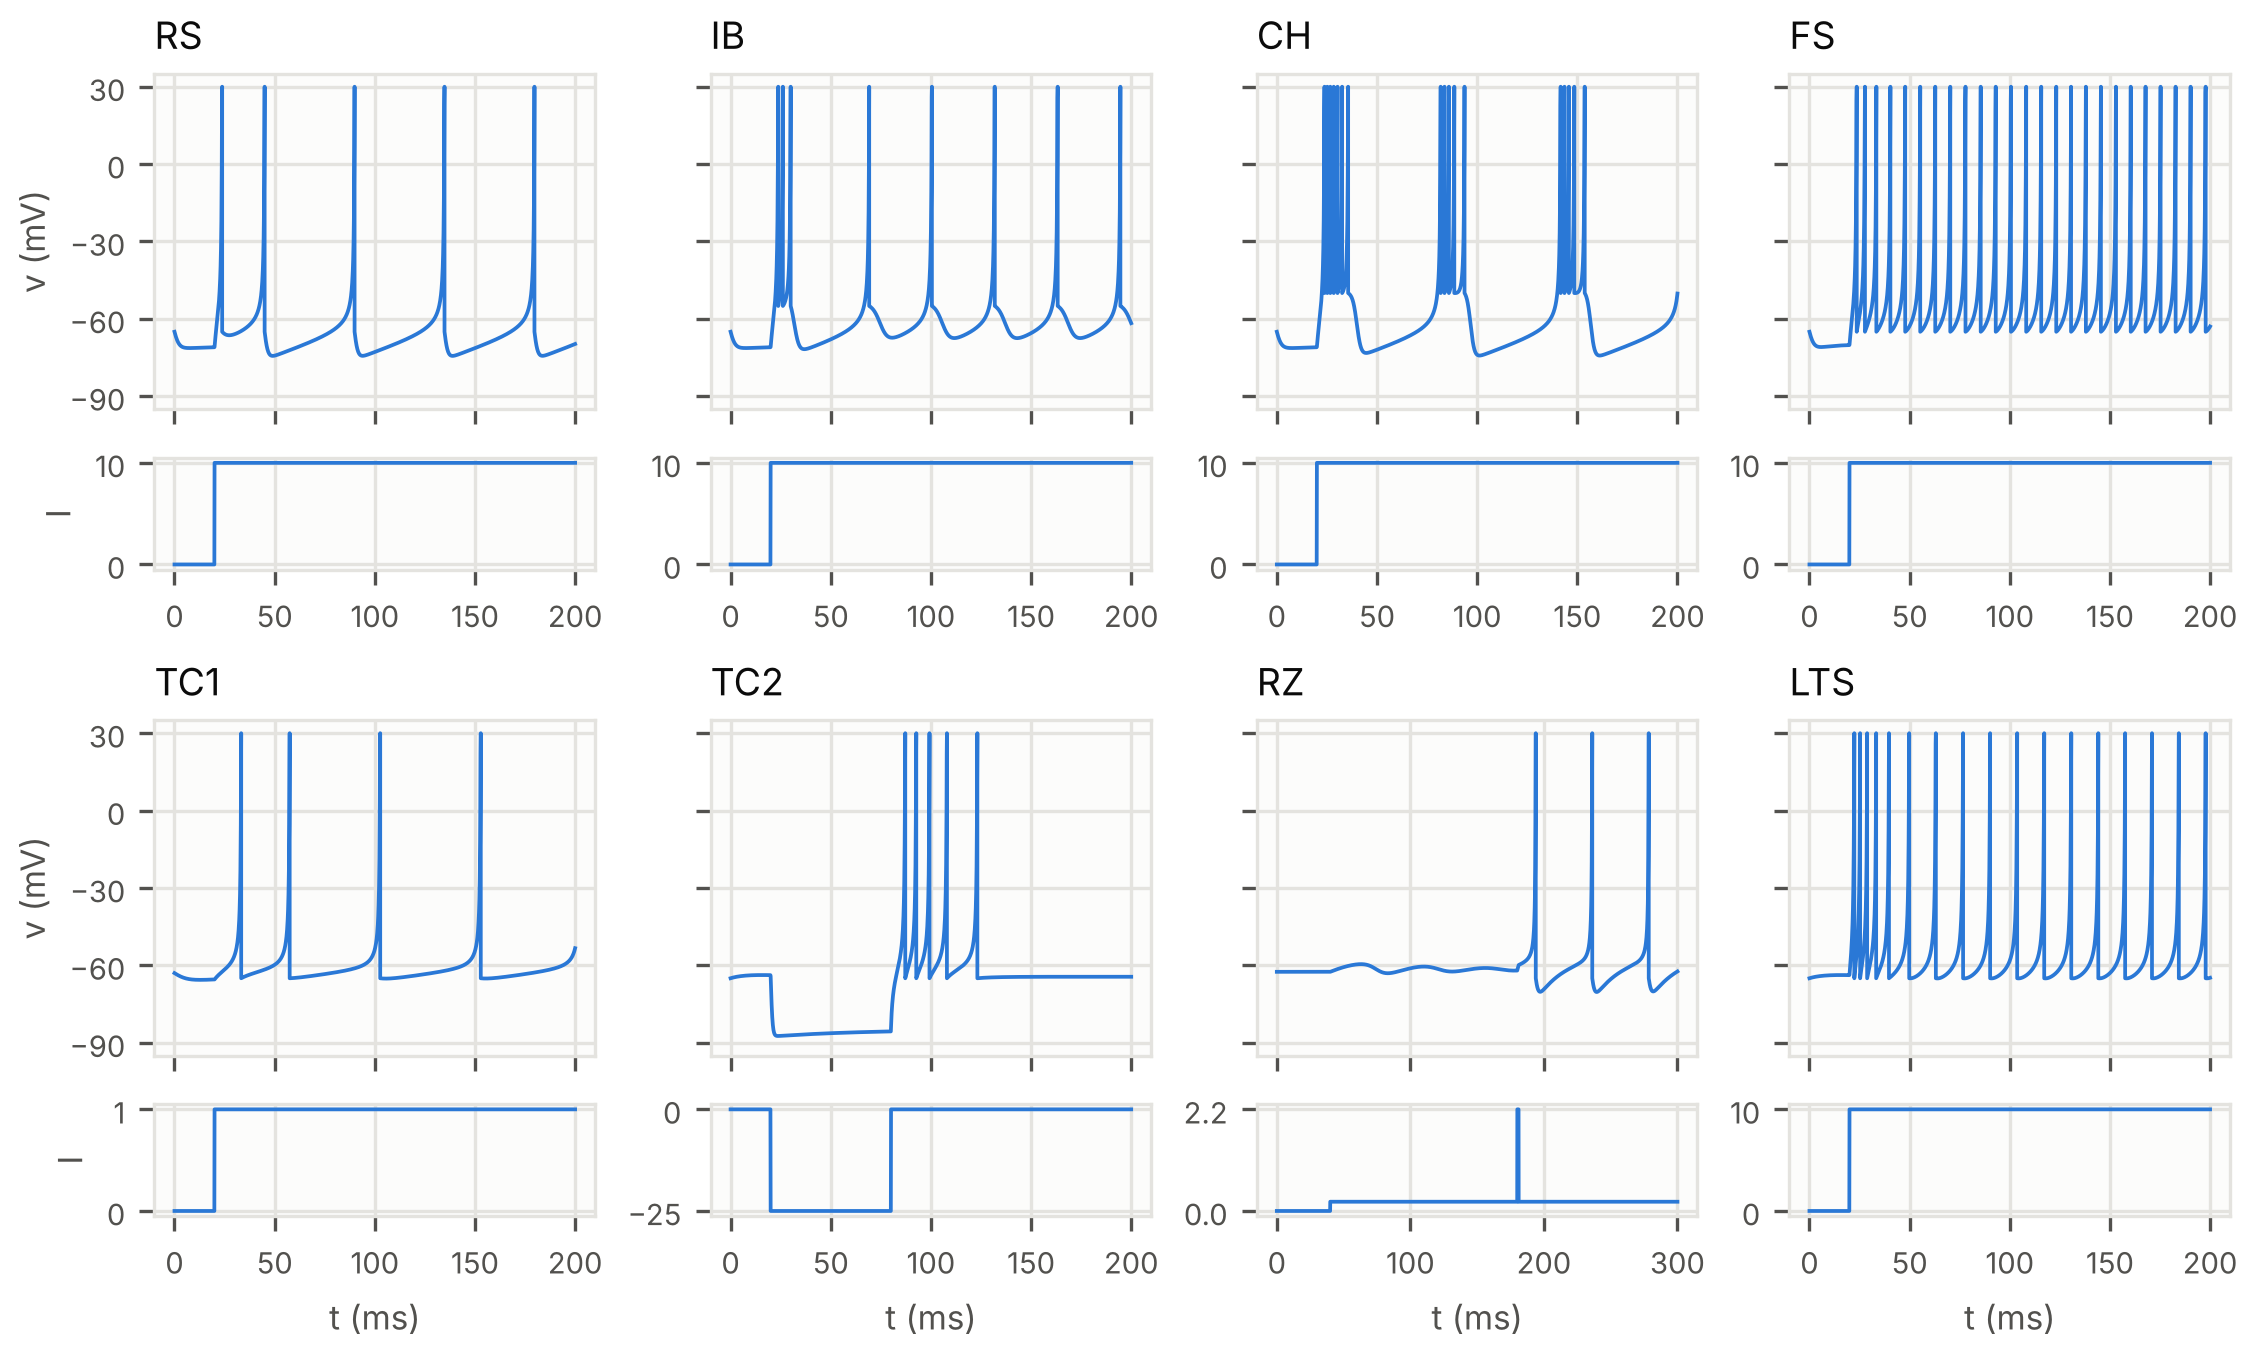
\includegraphics[width=0.86\textwidth]{f2_ocho_casos.png}
  \caption{Potencial de membrana $v(t)$ (paneles grandes) y corriente de entrada $I(t)$
  (tiras inferiores, rotuladas con sus valores extremos) para las ocho
  parametrizaciones de la Tabla~\ref{tab:parametros}, integradas con RK4 y
  $h=\num{0.1}$\,ms. Los paneles de $v$ comparten el eje vertical. Duración: 200\,ms
  (300\,ms en RZ).}
  \label{fig:tipos}
\end{figure*}

\textbf{Tipos de disparo.} Para reproducir la figura~2 de la Ref.~\cite{izhikevich2003}
usamos los parámetros de la Tabla~\ref{tab:parametros} y las corrientes de la consigna:
$I_1$, escalón de 10 en $t=20$\,ms; $I_2$, escalón de 1 en $t=20$\,ms; $I_3=-25$ en
$[20,80)$\,ms y 0 fuera; e $I_4$, \num{0.2} desde $t=40$\,ms más un pulso de \num{2.2}
en $[180,181)$\,ms. En la Figura~\ref{fig:tipos} se observa lo siguiente.
RS tiene un primer ISI de \num{21.2}\,ms y luego dispara regularmente cada
\num{44.9}\,ms. IB emite una ráfaga inicial de tres spikes (\num{23.8}--\num{30.0}\,ms)
seguida de spikes aislados cada $\approx\num{31.3}$\,ms. CH dispara ráfagas de siete,
cinco y cinco spikes que comienzan cada $\approx60$\,ms. FS emite 25 spikes: tras unos
pocos ISI cortos (\num{4.1}, \num{5.7} y \num{7.0}\,ms) se estabiliza en
$\approx\num{7.5}$\,ms ($\approx133$\,Hz). LTS también dispara a alta frecuencia, pero
su ISI crece de \num{2.9} a $\approx\num{13.5}$\,ms. En TC1 una corriente de sólo 1
alcanza para un disparo tónico lento (ISI de \num{24.2}, \num{45.2} y \num{50.2}\,ms).
En TC2 la neurona se hiperpolariza hasta $\approx\SI{-87}{\milivolt}$ durante el pulso
negativo y, al retirarlo, emite una ráfaga de rebote de cinco spikes entre \num{87.2} y
\num{123.2}\,ms, tras la cual vuelve al reposo. En RZ la corriente \num{0.2} produce
oscilaciones subumbrales amortiguadas de pocos mV ($v$ entre $-63$ y
$\SI{-59.5}{\milivolt}$), sin spikes, y el pulso de 1\,ms en $t=180$\,ms lo lleva al
disparo repetitivo (spikes en \num{193.9}, \num{236.2} y \num{278.5}\,ms). Barriendo
el instante $t_p$ del pulso entre 45 y 295\,ms, el pulso no dispara si llega en
$t_p\in[73,85]$ o $[123,130]$\,ms, y sí en el resto.

\begin{figure}[t]
  \centering
  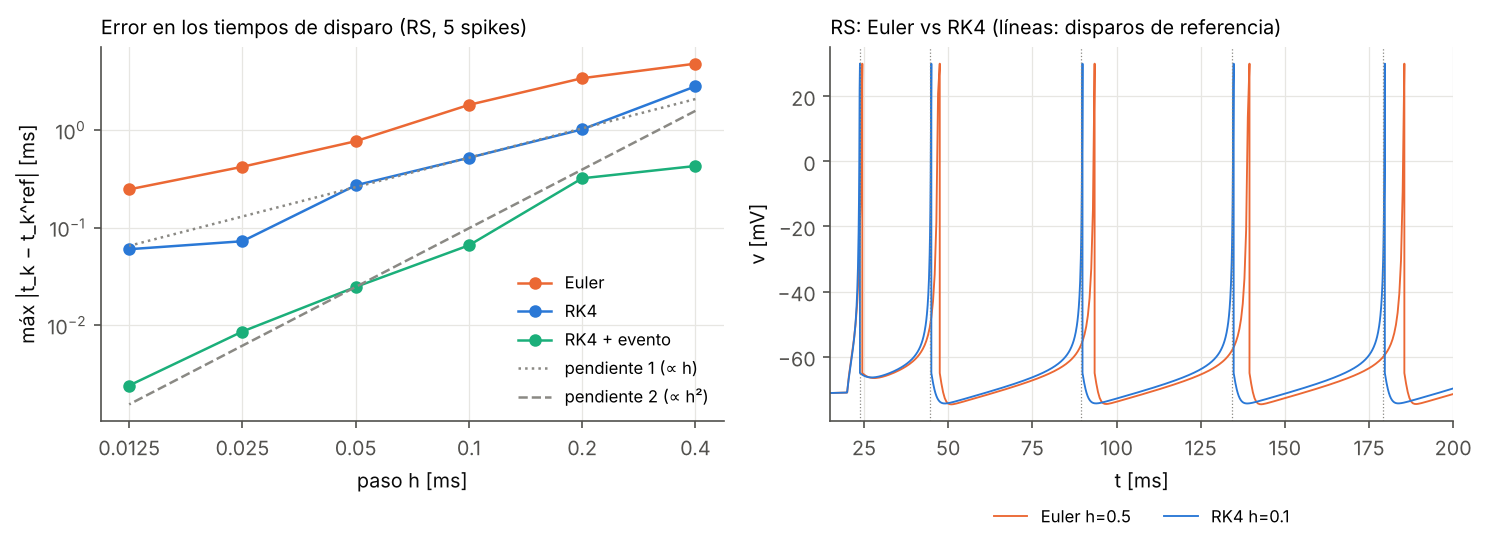
\includegraphics[width=\columnwidth]{f6_error.png}
  \caption{Izquierda: máximo error absoluto en los cinco tiempos de disparo de RS en
  función de $h$, para Euler, RK4 y RK4 localizando el cruce de \SI{30}{\milivolt} por
  interpolación lineal (``RK4 + evento''); en gris, rectas de pendiente 1 y 2.
  Derecha: $v(t)$ de RS con Euler ($h=\num{0.5}$\,ms, naranja) y RK4 ($h=\num{0.1}$\,ms,
  azul); las líneas punteadas son los disparos de referencia (\texttt{solve\_ivp},
  DOP853, tolerancia $10^{-11}$, con detección del cruce).}
  \label{fig:error}
\end{figure}

\textbf{Error numérico.} En la Figura~\ref{fig:error}, el error en los tiempos de
disparo de RK4 decrece aproximadamente como $h$ (pendiente~1), igual que el de Euler
pero con una constante menor: para $h=\num{0.1}$\,ms es \num{0.52}\,ms frente a
\num{1.82}\,ms de Euler. Localizando el cruce de \SI{30}{\milivolt} dentro del paso, el
error baja a \num{0.066}\,ms y decrece más rápido, con pendiente cercana a~2. Con Euler
y $h=\num{0.5}$\,ms los spikes se atrasan cada vez más respecto de la referencia.

\begin{figure*}[t]
  \centering
  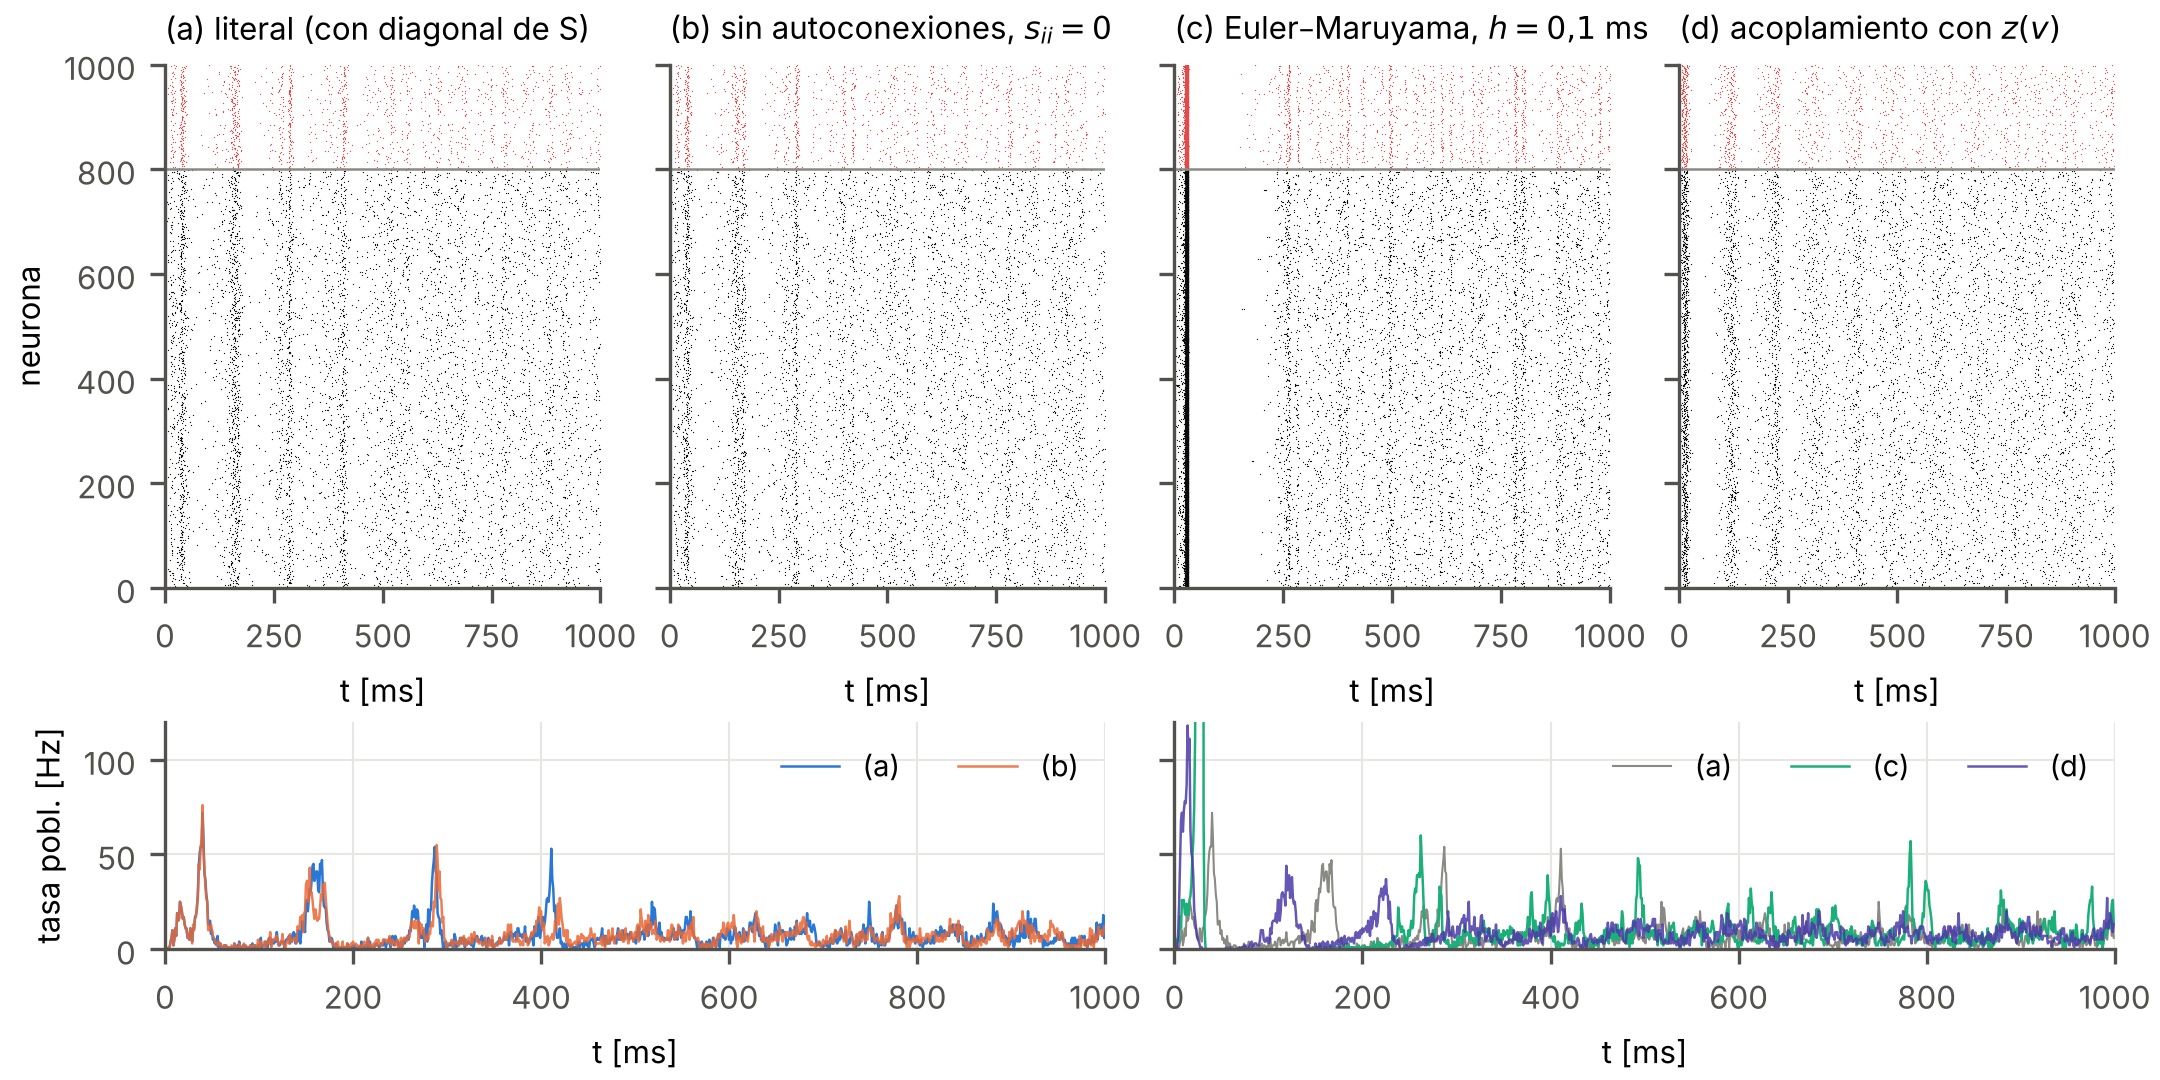
\includegraphics[width=0.92\textwidth]{f8_red_compacta.png}
  \caption{Red de 1000 neuronas durante 1000\,ms (semilla 2026). Arriba: rasters (cada
  punto es un spike; neuronas 1--800 excitatorias en negro y 801--1000 inhibitorias en
  rojo) de (a) la traducción literal del Matlab del artículo, (b) la misma red con
  $s_{ii}=0$, (c) la variante de Euler--Maruyama y (d) la variante con acoplamiento
  continuo $z(v)$. Abajo: tasa poblacional (spikes por neurona en bins de 1\,ms,
  en Hz); a la izquierda (a) y (b), a la derecha (a) en gris, (c) y (d).}
  \label{fig:red}
\end{figure*}

\textbf{Red de 1000 neuronas.} En la Figura~\ref{fig:red}(a) se observa actividad
asincrónica de fondo interrumpida por episodios de sincronización: bandas verticales
en las que gran parte de la población dispara a la vez, con picos de la tasa
poblacional en $\approx40$, 160, 290 y 410\,ms. El primero ocurre al arrancar, con todas
las neuronas en $v=\SI{-65}{\milivolt}$. Después de $\approx450$\,ms las bandas son más
débiles. La red literal emite \num{7765} spikes, con tasa media de \num{7.77}\,Hz
(\num{7.82}\,Hz las excitatorias y \num{7.57}\,Hz las inhibitorias), y el espectro de
la tasa poblacional para $t>100$\,ms tiene su máximo en $\approx\num{7.8}$\,Hz.
Con la misma semilla y sin autoconexiones [Fig.~\ref{fig:red}(b)] la red emite
\num{7561} spikes (\num{7.56}\,Hz). Los episodios grandes aparecen en tiempos parecidos
($\approx40$, 150, 290 y 400--420\,ms), con amplitudes algo distintas, mientras que los
spikes individuales difieren. Repitiendo la comparación con 20 semillas ($t>100$\,ms),
la tasa media es $\num{7.19}\pm\num{0.13}$\,Hz con diagonal y
$\num{7.17}\pm\num{0.13}$\,Hz sin ella; la diferencia es $\num{0.02}\pm\num{0.12}$\,Hz.

En la variante de Euler--Maruyama [Fig.~\ref{fig:red}(c)] hay un episodio inicial muy
intenso entre \num{3.5} y \num{33.4}\,ms, en el que cada neurona dispara unas 24 veces
(\num{24357} spikes), seguido de casi 200\,ms de silencio; luego aparece actividad
asincrónica con bandas, con tasa media de \num{8.23}\,Hz para $t>100$\,ms. Con
acoplamiento continuo $z(v)$ [Fig.~\ref{fig:red}(d)] también hay fondo asincrónico y
bandas, más anchas al principio (\num{8798} spikes; \num{8.34}\,Hz para $t>100$\,ms,
frente a \num{7.54}\,Hz de la red literal en el mismo intervalo).

% =====================================================================
\section{Discusión}
\textbf{Tipos de disparo.} Las simulaciones reproducen cualitativamente los ocho
paneles de la figura~2 de la Ref.~\cite{izhikevich2003}, y cada patrón coincide con la
descripción del artículo. RS muestra adaptación de frecuencia (spikes con período corto
que luego se alarga), que el artículo atribuye al reseteo profundo ($c=-65$) y al salto
grande de $u$ ($d=8$). En IB, el reseteo alto ($c=-55$) y $d=4$ producen una ráfaga
estereotipada seguida de spikes simples: durante la ráfaga $u$ se acumula hasta que
conmuta la dinámica de ráfaga a disparo simple. En CH, el reseteo aún más alto
($c=-50$) con $d=2$ da ráfagas repetidas de spikes muy próximos; nuestra frecuencia
entre ráfagas ($\approx17$\,Hz) está por debajo de los 40\,Hz que el artículo menciona
como máximo posible. FS, con recuperación rápida ($a=\num{0.1}$), dispara a muy alta
frecuencia prácticamente sin adaptación una vez pasados los primeros spikes; LTS
($b=\num{0.25}$, umbral bajo) dispara a alta frecuencia pero con adaptación notoria,
que es lo que distingue a ambas interneuronas inhibitorias. TC presenta sus dos
regímenes: disparo tónico al despolarizarla desde el reposo (TC1) y ráfaga de rebote
tras una hiperpolarización hasta $\approx-87$\,mV (TC2), cerca de los $\approx-90$\,mV
que indica el artículo. RZ ($a=\num{0.1}$, $b=\num{0.26}$) muestra las oscilaciones
subumbrales amortiguadas y la biestabilidad entre reposo y disparo repetitivo: un
estímulo breve, aplicado en el momento adecuado, conmuta de un estado al otro. El
barrido de $t_p$ muestra que la conmutación depende de la fase de la oscilación en que
llega el pulso: es una respuesta resonante y no de umbral fijo. Las diferencias
cuantitativas con el artículo (número de spikes, latencias) son esperables, porque el
artículo no tabula las corrientes: aquí usamos los protocolos de la consigna, que
además fijan $v(0)$, del que dependen algunos casos.

\textbf{Paso de integración y reseteo.} RK4 es de orden~4 entre spikes, pero el reseteo
se detecta recién en el primer punto de la grilla con $v\geq\SI{30}{\milivolt}$: cada
tiempo de disparo queda redondeado al paso siguiente, un error $\mathcal O(h)$ que se
arrastra a los spikes posteriores porque el reseteo parte de un estado corrido. Esto
explica la pendiente~1 de la Fig.~\ref{fig:error} y que RK4 sólo mejore a Euler en la
constante. Localizar el cruce dentro del paso recupera precisión, con un orden
limitado por la interpolación lineal. Otras fuentes de error son la rigidez del
término $v^2$ cerca del pico, donde $v$ crece explosivamente y con $h$ grande puede
pasarse mucho de 30\,mV dentro de un paso, y la sensibilidad de los casos cercanos a
una bifurcación, como RZ, donde un error pequeño puede cambiar el régimen de la
trayectoria. Por eso el paso $h$ y el tratamiento del reseteo importan tanto como el
orden nominal del método.

\textbf{Red.} La traducción literal reproduce lo que el artículo describe para su
figura~3: actividad asincrónica con tasas medias de $\approx8$\,Hz y episodios
ocasionales de sincronización. Los episodios grandes se repiten cada $\approx120$\,ms,
lo que coincide con el máximo espectral en $\approx\num{7.8}$\,Hz, cerca de la banda
$\alpha$ ($\approx10$\,Hz) que reporta el artículo. Las autoconexiones aportan a cada
neurona un único peso (a lo sumo \num{0.5} si es excitatoria, o hasta $-1$ si es
inhibitoria) frente a la suma de las entradas de toda la red: quitarlas cambia los
spikes individuales, pero no la tasa media (la diferencia sobre 20 semillas es mucho
menor que su dispersión) ni la estructura de los episodios sincrónicos. Concluimos que
la diagonal de $S$ no modifica cualitativamente la dinámica.

En la variante de Euler--Maruyama, los saltos sinápticos se aplican cada
\num{0.1}\,ms; inferimos que, con todas las neuronas partiendo del mismo estado, la
primera descarga sincrónica genera saltos que vuelven a superar 30\,mV en los pasos
siguientes, lo que produce el episodio inicial de $\approx24$ spikes por neurona.
Superado ese transitorio, la dinámica (tasa $\approx8$\,Hz con bandas) es comparable a
la del original. La variante con $z(v)$ es un modelo distinto: la entrada sináptica no
depende de los eventos de disparo sino del potencial de todas las neuronas en todo
momento, por lo que incluye un fondo permanente que eleva la tasa
($\approx\num{8.3}$ frente a $\approx\num{7.5}$\,Hz) y cambia la forma de los
episodios; no reproduce la figura~3 y sólo sirve como comparación.

\section*{Agradecimientos}
A los docentes Francisco Tamarit, Juan Perotti, Tristán Osán y Franco Milana, por la
guía de prácticos y las clases en las que se basa este trabajo.

% =====================================================================
\begin{thebibliography}{9}\small
\setlength{\itemsep}{0pt}
\bibitem{izhikevich2003}
  E.~M. Izhikevich, ``Simple model of spiking neurons,''
  \emph{IEEE Trans.\ Neural Netw.} \textbf{14}(6), 1569--1572 (2003).
\bibitem{izhikevich2007}
  E.~M. Izhikevich, \emph{Dynamical Systems in Neuroscience: The Geometry of
  Excitability and Bursting}, MIT Press, Cambridge, MA (2007).
\bibitem{hodgkin1952}
  A.~L. Hodgkin y A.~F. Huxley, ``A quantitative description of membrane
  current and its application to conduction and excitation in nerve,''
  \emph{J.\ Physiol.} \textbf{117}(4), 500--544 (1952).
\bibitem{dayan2001}
  P.~Dayan y L.~F. Abbott, \emph{Theoretical Neuroscience: Computational and
  Mathematical Modeling of Neural Systems}, MIT Press, Cambridge, MA (2001).
\bibitem{lapicque1907}
  L.~Lapicque, ``Recherches quantitatives sur l'excitation électrique des nerfs
  traitée comme une polarisation,'' \emph{J.\ Physiol.\ Pathol.\ Gén.} \textbf{9},
  620--635 (1907).
\bibitem{em}
  Euler--Maruyama method,
  \url{https://en.wikipedia.org/wiki/Euler\%E2\%80\%93Maruyama_method}.
\end{thebibliography}

\end{document}
